% Writed by: Stavros Papantonakis
%
%!TEX TS-program = xelatex
%!TEX encoding = UTF-8 Unicode
%

\setcounter{section}{1}
\section{Σύνδεση με την θεματολογία των ασκήσεων}

\noindent
Παρατηρούμε ότι οι παραπάνω ευπάθειες χρησιμοποιούν την αδυναμία του συστήματος να φιλτράρει και να εξουδετερώσει την JavaScript που προστίθεται στα διαφορά section του συστήματος τους από χρήστες. Επιτρέποντας έτσι πιθανών κακόβουλες ενέργειες που μπορεί να προκύψουν και μη ορθή χρίση του συστήματος. 

\noindent
Προσθέτοντας κάποιος χρήστης μια εικόνα στο email attachment όπου στο onload φορτώνει κάποιον JavaScript κακόβουλο κώδικα που ενδεχομένως έχει ανεβάσει σε κάποιων απομακρυσμένο server οπός αντίστοιχα κάναμε και στο πρώτο μέρος της τέταρτης εργαστηριακής άσκησης και αποστείλει το email στο ανυποψίαστο θύμα. Θα έχει ως αποτέλεσμα ανοίγοντας το, ο κακόβουλος κώδικας να εκτελεστεί στον browser του θύματος και να προκαλέσει μη επιθυμητές ενέργειες οπός η υποκλοπή cookie session η άλλων δεδομένων του ανυποψίαστου χρήστη. 

\noindent
Η συγκεκριμένοι τύποι ευπαθείας (CVE-2004-1935 και CVE-2005-0945)\footnote{Προσθήκη} υπόκεινται στην κατηγορία των XSS (Cross Site Scripting) αντίστοιχες με αυτές που εξετάσαμε στην εργαστηριακή άσκηση 4. Παραδείγματος χάριν θα μπορούσε και στης δυο περιπτώσεις να δημιουργηθεί κάτι αντίστοιχο του Samyworm που υλοποιήσαμε στο εργαστήριο. 

\noindent
Στο πρώτο χρησιμοποιώντας μια εικόνα στο attachment ενός email οπού στο attribute onload θα φορτώσει των κακόβουλο κώδικα, ο οποίος θα σταλθεί στα επόμενα θύματα χρησιμοποιώντας τα πιθανόν αποθηκευμένα email του κάθε χριστή. Αντίστοιχα στο δεύτερο θα μπορούσε να αναπαράγετε και να δημοσιεύετε από κάθε χρήστης που βλέπει είτε ένα link είτε μια εικόνα στο comment section της web ιστοσελίδας. 




\section{Τεχνική περιγραφή και ανάλυση με παραδείγματα}

\subsection{Τεχνική περιγραφή}

\noindent
Ας ξεκινήσουμε να προσεγγίζουμε λίγο πιο συγκεκριμένα την αδυναμία (CWE-83)\footnote{Προσθήκη} που αναφέραμε παραπάνω.  Αρχικά ένας επιτιθέμενος που εκμεταλλεύεται την συγκεκριμένη ευπάθεια καθώς και όλες όσες υπόκεινται στην κατηγορία των XSS, προσπαθεί να εμφυτεύσει στο αντίστοιχο λογισμικό, συνήθως web εφαρμογή κώδικα ο οποίος θα εκτελεστεί στον browser του θύματος σαν να ήταν εξαρχής μέρος της όταν έρθει σε επαφή με αυτόν. 

\noindent
Ο επιτιθέμενος με αυτόν τον τρόπο μπορεί να στείλει σε ένα ανυποψίαστο χρήστη το script με τον κακόβουλο κώδικα. Ο χρήστης δεν έχει την παραμικρή ιδέα για το ότι ο συγκεκριμένος κώδικας δεν είναι έμπιστος καθώς προέρχεται από μια έμπιστη ιστοσελίδα. Έτσι το κακόβουλο script εκτελείται στον browser του χρήστη με αποτέλεσμα να έχει πρόσβαση σε cookies, sessions και άλλες ευαίσθητες πληροφορίες που βρίσκονται στον browser του χρήστη και χρησιμοποιούνται από το συγκεκριμένο site.

\subsection{Παραδείγματα}
\noindent
Ειδικότερα σε αυτήν την αδυναμία (CWE-83)\footnote{Προσθήκη} χρησιμοποιούνται εναλλακτικές μέθοδοι εμφύτευσης κώδικα στην ιστοσελίδα χωρίς να χρησιμοποιούνται τα script tags.
\begin{center}
			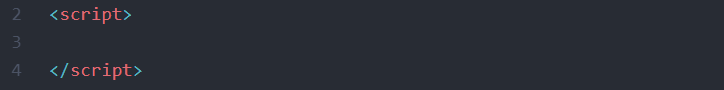
\includegraphics[width=1\textwidth]{image/1 script tags.PNG}		
\end{center}

\subsection{Ενναλακτική σύνταξη XSS}
\noindent
Ας δώσουμε μερικά παραδείγματα όπως την χρήση XSS του attribute onload,
\begin{center}
			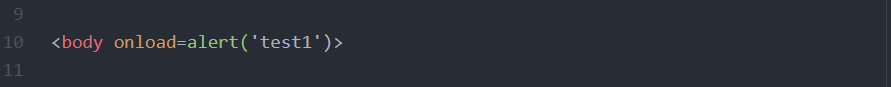
\includegraphics[width=1\textwidth]{image/2.PNG}		
\end{center}

\noindent
τα attributes onmouseover
\begin{center}
			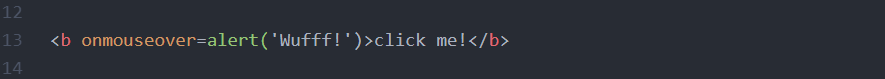
\includegraphics[width=1\textwidth]{image/3.PNG}		
\end{center}
\noindent
και onerror
\begin{center}
			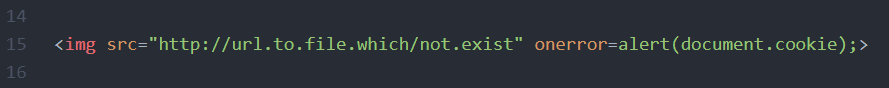
\includegraphics[width=1\textwidth]{image/4.PNG}		
\end{center}
\subsection{Χρήση XSS μέσω κωδικοποιημένου URI}
\noindent
Ακόμα και αν ένα site κάνει filtering υπάρχει η πιθανότητα να κωδικοποιηθεί σε UTF-8 και να περαστεί στο img tag.
\begin{center}
			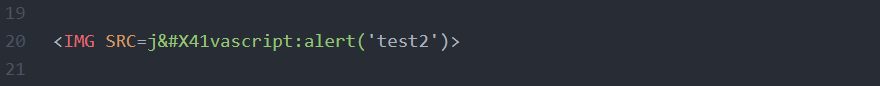
\includegraphics[width=1\textwidth]{image/5.PNG}		
\end{center}
\noindent
Άλλες μέθοδοι υπεκφυγής φιλτραρίσματος είναι
\subsection{XSS εικόνα χρησιμοποιώντας JavaScript directive}
\begin{center}
			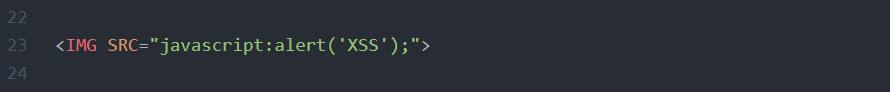
\includegraphics[width=1\textwidth]{image/6.PNG}		
\end{center}
\subsection{Χρήση εισαγωγικά και ερωτηματικά}
\begin{center}
			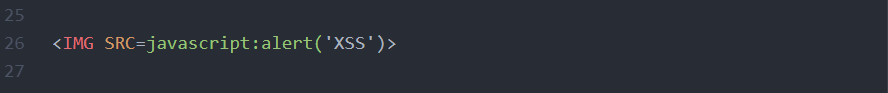
\includegraphics[width=1\textwidth]{image/7.PNG}		
\end{center}
\subsection{Χρήση case insensitive γραφής}
\begin{center}
			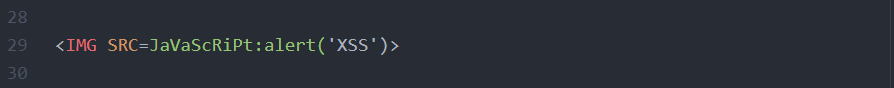
\includegraphics[width=1\textwidth]{image/8.PNG}		
\end{center}
\subsection{Χρήση HTML χαρακτήρων}
\noindent
Απαιτούνται οι χαρακτήρες (;) για αυτή την περίπτωση.
\begin{center}
			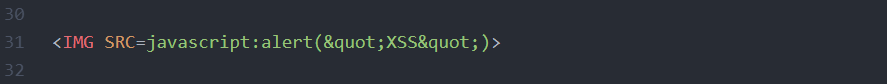
\includegraphics[width=1\textwidth]{image/10.PNG}		
\end{center}
\subsection{Χρήση του χαρακτήρα (`)}
\noindent
Χρησιμοποιώντας τον χαρακτήρα (`) έτσι ώστε να περικλείει το script string, τα XSS filters  σε πολλές περιπτώσεις δεν τον αναγνωρίζουν.\footnote{Αλλαγή}
\begin{center}
			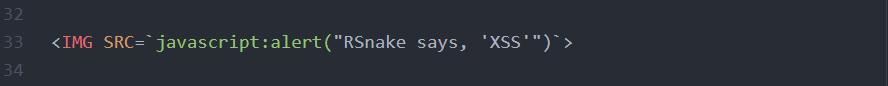
\includegraphics[width=1\textwidth]{image/11.PNG}		
\end{center}

\subsection{Λάθος σύνταξη HTML tags}
\begin{center}
			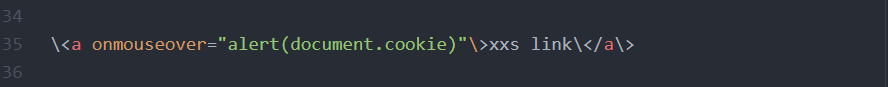
\includegraphics[width=1\textwidth]{image/12.PNG}		
\end{center}
\subsection{Λάθος σύνταξη HTML IMG tag}
\begin{center}
			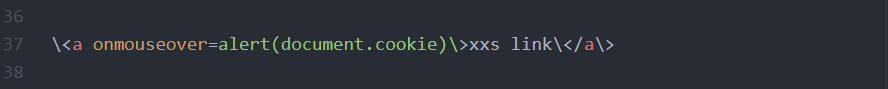
\includegraphics[width=1\textwidth]{image/13.PNG}		
\end{center}
\subsection{fromCharCode}
\noindent
Ακόμα και να φιλτράρονται όλοι οι χαρακτήρες εισαγωγικών μπορούμε να δημιουργήσουμε οποιαδήποτε συμβολοσειρά επιθυμούμε με αυτήν την συνάρτηση της JavaScript
\begin{center}
			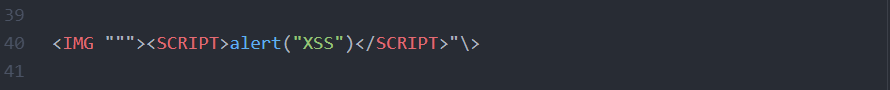
\includegraphics[width=1\textwidth]{image/14.PNG}		
\end{center}
\subsection{Χρήση του χαρακτήρα (\#) στο SRC attribute }
\begin{center}
			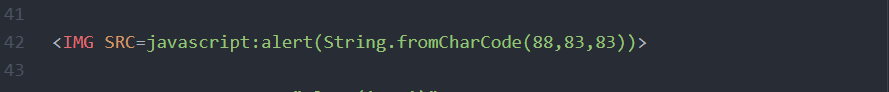
\includegraphics[width=1\textwidth]{image/15.PNG}		
\end{center}
\subsection{Κενό SRC attribute}
\begin{center}
			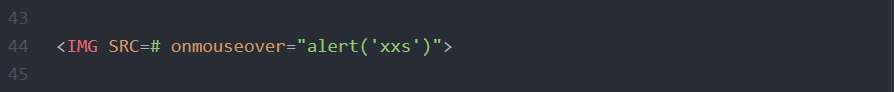
\includegraphics[width=1\textwidth]{image/16.PNG}		
\end{center}
\subsection{Χρήση tag με παράληψη του SRC attribute}
\begin{center}
			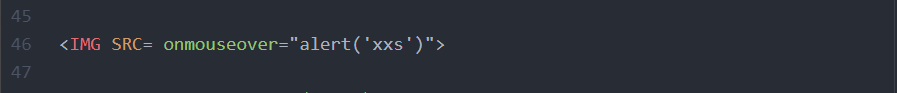
\includegraphics[width=1\textwidth]{image/17.PNG}		
\end{center}
\subsection{Χρήση του attribute onerror}
\begin{center}
			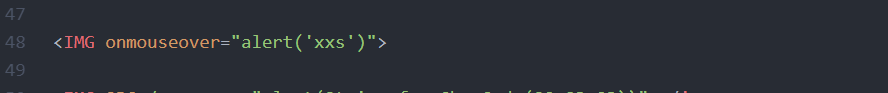
\includegraphics[width=1\textwidth]{image/18.PNG}		
\end{center}
\subsection{Χρήση του attribute onerror με κωδικοποιημένο script string}
\begin{center}
			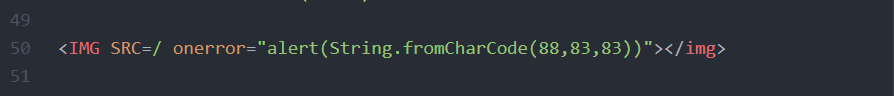
\includegraphics[width=1\textwidth]{image/19.PNG}		
\end{center}
\subsection{Κωδικοποίηση JavaScript Directive με δεκαδικούς html χαρακτήρες}
\begin{center}
			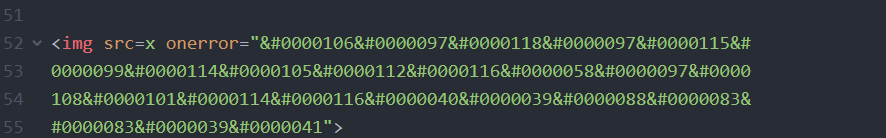
\includegraphics[width=1\textwidth]{image/20.PNG}		
\end{center}
\subsection{Κωδικοποίηση JavaScript Directive με δεκαδικούς html χαρακτήρες χωρίς ερωτηματικά }
\begin{center}
			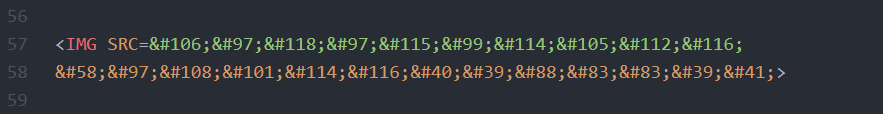
\includegraphics[width=1\textwidth]{image/21.PNG}		
\end{center}
\subsection{Κωδικοποίηση JavaScript Directive με δεκαεξαδικούς html χαρακτήρες}
\begin{center}
			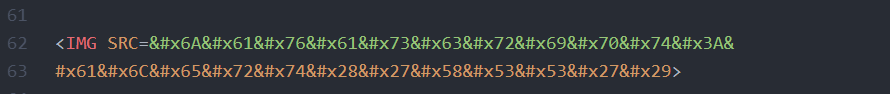
\includegraphics[width=1\textwidth]{image/22.PNG}		
\end{center}
\noindent
Παρατηρούμε ότι δεν υπάρχει ένας και μοναδικός τρόπος εμφύτευσης κώδικα JavaScript  σε μια ιστοσελίδα. Αντιθέτως υπάρχει πληθώρα τροπών και μεθόδων που μπορούν να οδηγήσουν σε ένα σενάριο XSS. Αυτό μας οδηγεί στο συμπέρασμα ότι η δουλειά ενός XSS φίλτρου είναι πολύ δύσκολη και πιθανόν ακατόρθωτη σε μερικές περιπτώσεις. Έχοντας ως συνέπεια την αύξηση της πιθανότητας κάποιο από τα ενδεχόμενα σενάρια να μην ελεγχθεί είτε να ελεγχθεί, εσφαλμένα οδηγώντας έτσι την web εφαρμογή σε ένα XSS Attack σενάριο.

\section{Περιστατικά και συνέπειες που σχετίζονται την αδυναμία (CWE-83)}


\subsection{Περιστατικά}
\noindent
Όπως αναφέραμε και στην αρχή υπάρχουν αρκετά περιστατικά που σχετίζονται με την παραπάνω αδυναμία. Στην συνεχεία θα αρχίσουμε να αναλύουμε αυτά που μας φανήκαν πιο ενδιαφέροντα. Τo CVE-2004-1935 αναφέρει μια ευπάθεια XSS στο SCT Campus Pipeline όπου επιτρέπει την JavaScript  σε tags όπως τα onload, onmouseover, κλπ ως συνημμένα σε email, και το CVE-2005-0945 όπου μιλάει για ευπάθεια XSS στο ACS Blog 1.1.1 οπού επιτρέπει την εισαγωγή JavaScript στο comment section μέσω του onmouseover attribute στα tags link, mail, img.  

\subsection{CVE-2004-1935}

\noindent
Αναφορικά το SCT Campus Pipeline ήταν μια διαδικτυακή πλατφόρμα που είχε επιλεχθεί να χρησιμοποιήστε σε πάνω από 175 ιδρύματα. Το οποίο χρησιμοποιούνταν για την κοινωνικοποίηση και την βελτίωση της απόδοσης των φοιτητών, παρέχοντας τους πρόσβαση σε πληροφορίες, υπηρεσίες και κοινότητες.


\noindent
Το τμήμα χειρισμού του email αυτού του λογισμικού εμφάνιζε στο εσωτερικό του email ορισμένα συνημμένα όπως html, bmp, jpg, gif, κλπ. Ενώ όμως έκανε πολύ καλή δουλεία στο φιλτράρισμα των script από τα αρχεία html άφηνε απείραχτα κάποια events όπως το onload(), onmouseover(), onclick(),κλπ. 

\noindent
Όπως καταλαβαίνουμε αυτό είναι τεράστιο πρόβλημα καθώς ο ενδεχόμενος κακόβουλος κώδικας που μπορεί να καλείται από αυτά τα events θα έχει τα ιδία δικαιώματα με τον χρήστη που περιηγείται στο email του. Το πράγμα γίνετε ακόμα χειρότερο γιατί η εφαρμογή χρησιμοποιεί συναρτήσεις JavaScript για την υλοποίηση όλων των λειτουργιών που διαθέτει. 

\noindent
Συνεπώς αυτό καθιστούσε δυνατόν την εκτέλεση εντολών όπως delete message() στο <body onload=”deletemessage()”> με αποτέλεσμα τη διαγράφη του email μαζί με τον κώδικα html που έχει επισυναφθεί σε αυτό. Ακόμα αλλάζοντας την σελίδα στον χρήστη με την <body onload= ”location.replace(‘site’)”> θα μπορούσαμε να εκτελέσουμε τον πιθανόν κακόβουλο κώδικα που  θα είχαμε προετοιμάσει ή να εφαρμόσουμε οποιαδήποτε μέθοδο scripting επιθυμούσαμε.

\noindent
Αυτό το κενό ασφάλειας μπορεί να οδηγήσει σε ένα συνημμένο html που έχει πλήρη έλεγχο του email λογαριασμού των θυμάτων. Εφόσον ο επιτιθέμενος θα είχε ρυθμίσει τα session των χρηστών, θα μπορούσε ενδεχομένως να εκτελέσει οποιαδήποτε εντολή μπορούσε να χρησιμοποιήσει ο συγκεκριμένος λογαριασμός, όπως την προβολή βαθμών του φοιτητή κλπ.

\noindent
Μερικά παραδείγματα που εκμεταλλεύονται την ευπάθεια του συγκεκριμένου site είναι τα παρακάτω: 
\begin{center}
			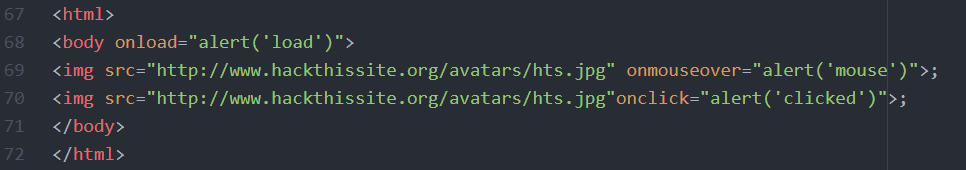
\includegraphics[width=1\textwidth]{image/23.PNG}		
\end{center}
\noindent
Το συγκεκριμένο exploit διαγράφει το ενδεχόμενο μήνυμα.
\begin{center}
			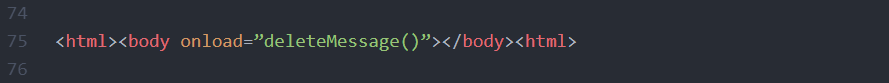
\includegraphics[width=1\textwidth]{image/24.PNG}		
\end{center}
\noindent
Με το παρακάτω exploit δημιουργούμε ένα νέο μήνυμα email με ότι περιεχόμενο θέλουμε.
\begin{center}
			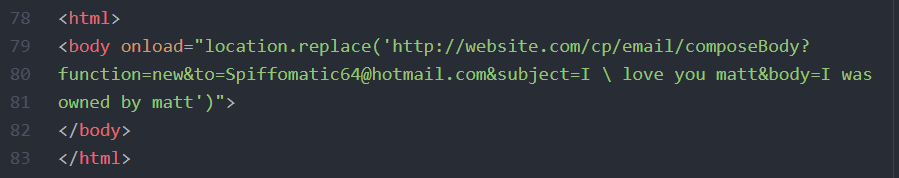
\includegraphics[width=1\textwidth]{image/25.PNG}		
\end{center}
\noindent
Η δημιουργία ενός ψευδούς session timeout screen με μια login form θα αποτελούσε εξίσου μεγάλο πρόβλημα. αυτό θα οδηγούσε τους χρήστες να πληκτρολογήσουν τα ακαδημαϊκά τους στοιχεία, πέφτοντας έτσι στην παγίδα του επιτιθέμενου, υποκλέπτοντας τους, ευαίσθητες πληροφορίες και ότι άλλο μπορεί να συνεπάγεται με αυτό.
\begin{center}
			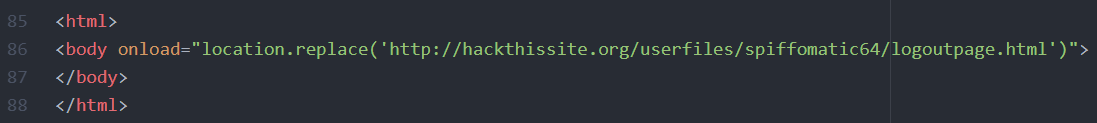
\includegraphics[width=1\textwidth]{image/26.PNG}		
\end{center}
\noindent
Η συγκεκριμένη ευπάθεια δημοσιεύτηκε στο CVE Details στις 15-04-2004, marc.info στις 15-04-2004 και ώρα 16:36:50, SecurityFocus 15-04-2004 και ώρα 12:00ΑΜ και τέλος  στο ΙΒΜcloud στις 15-04-2004. 

\noindent
Ο βαθμός σοβαρότητας διαφέρει στα διαφορά sites. Για παράδειγμα στο \textbf{ΙΒΜcloud} έχει 
\\
\\
\begin{tabular}{rl}
\hline
CVSS 1.0 Base Score: & 2.8 \\
Access Vector: 	& Remote \\
Access Complexity: &	High \\ 
Authentication: & Not Required \\
Confidentiality Impact: & None \\
Integrity Impact: & Partial \\ 
Availability Impact: & None \\
\hline
\end{tabular}


\noindent
Ενώ στο \textbf{CVE Details} έχει 


\begin{tabular}{rl}
\hline
CVSS Score: & 	4.3\\
Confidentiality Impact: & \noindent None \\
Integrity Impact: & Partial \\
Availability Impact:  &	None \\
Access Complexity: &	Medium \\
Authentication: 	& Not required \\
Gained Access: 	& None\\
Vulnerability Type(s): & 	Cross Site Scripting	\\
CWE ID: &	CWE id is not defined \\
\hline
\end{tabular}


\noindent
Τέλος σύμφωνα με το CVE Details η συγκεκριμένη ευπάθεια υπήρχε στο λογισμικό Campus Pipeline της Sct Corporation για τις εκδόσεις 1.0, 2.0, 2.1, 2.2, 3.0, 3.1, 3.2

\subsection{CVE-2005-0945}
\noindent 
Η συγκεκριμένη ευπάθεια δοκιμάστηκε στη έκδοσή (V1.1.1) του ACS Blog. Όπως είπαμε και παραπάνω στο comment section του ACS Blog υπήρχε η πιθανότητα εκτέλεσης μιας επίθεσης XSS μέσω των link,mail, img tags, λόγω έλλειψης φιλτραρίσματος στα μονά εισαγωγικά και στα κενά μέσα στα tags. 

\noindent
Εδώ παρατηρούμε ότι ισχύουν πάνω κάτω τα ίδια πράγματα με την προηγουμένη ευπάθεια, δηλαδή κάποιος κακόβουλος χρηστής θα μπορούσε να προσθέσει τον κακόβουλο κώδικα του στο onload του tag μιας εικόνας και να την προωθήσει στο comment section, με αποτέλεσμα ο κακόβουλος κώδικας να εκτελεστεί σε οποιονδήποτε browser εμφανίσει το εν λόγω comment.

\noindent
Ας δούμε μερικά παραδείγματα σεναρίων που μπορούν να εμφυτεύσουν εκτελέσιμο κώδικα στο comments section.

\begin{center}
			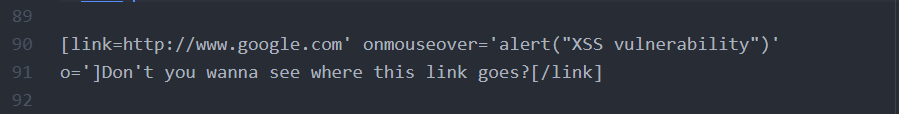
\includegraphics[width=1\textwidth]{image/27.PNG}		
\end{center}

\begin{center}
			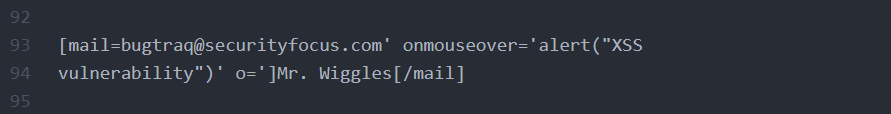
\includegraphics[width=1\textwidth]{image/28.PNG}		
\end{center}

\begin{center}
			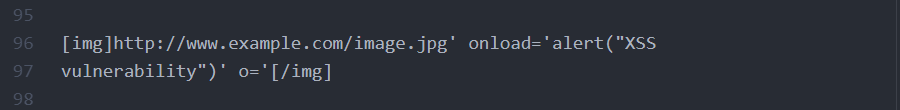
\includegraphics[width=1\textwidth]{image/29.PNG}		
\end{center}

\begin{center}
			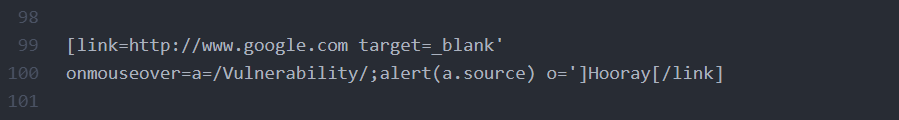
\includegraphics[width=1\textwidth]{image/30.PNG}		
\end{center}

\noindent
Η συγκεκριμένη ευπάθεια δημοσιεύτηκε στο CVE Details στις 02-05-2005, marc.info στις 28-03-2005 και ώρα 23:15:34, SecurityFocus 28-03-2005 και ώρα 12:00ΑΜ, ΙΒΜcloud στης 28-03-2005, και τέλος στο NIST 05-02-2005. 

\noindent
Βαθμός σοβαρότητας στα διαφορά sites:



\textbf{NIST}

\begin{tabular}{rl}
\hline
CVSS Base Score: & 	4.3\\
Impact Subscore: & 2.9 \\ 
Exploitability Subscore: & 8.6\\
CVSS Temporal Score: &    NA\\
CVSS Environmental Score: &  NA\\
Modified Impact Subscore: &    NA\\
Overall CVSS Score: &    4.3\\
\hline
\end{tabular}

\textbf{ΙΒΜcloud}
\\
\\
\begin{tabular}{rl}
\hline
CVSS 1.0 Base Score: & 2.8 \\
Access Vector: 	& Remote \\
Access Complexity: &	High \\ 
Authentication: & Not Required \\
Confidentiality Impact: & None \\
Integrity Impact: & Partial \\ 
Availability Impact: & None \\
\hline
\end{tabular}


\textbf{CVE Details}\\ \\
\begin{tabular}{rl}
\hline
CVSS Score: & 	4.3\\
Confidentiality Impact: & \noindent None \\
Integrity Impact: & Partial \\
Availability Impact:  &	None \\
Access Complexity: &	Medium \\
Authentication: 	& Not required \\
Gained Access: 	& None\\
Vulnerability Type(s): & 	Cross Site Scripting	\\
CWE ID: &	CWE id is not defined \\
\hline
\end{tabular}


\noindent
Οι συγκεκριμένες ευπάθειες εάν βρισκόταν σε πιο διαδεδομένες web εφαρμογές θα μπορούσαν να οδηγήσουν σε ένα worm με πιθανόν πολύ μεγαλύτερή ταχύτητα εξαπλώσεις από το Sumy worm λόγω του ότι το CVE-2004-1935 περιγράφει ευπάθεια μέσω email που επιτρέπει στον επιτιθέμενο να τοποθετήσει κακόβουλο κώδικα στο εσωτερικό του email και να το αποστείλει σε μια λίστα χρηστών οπού ανοίγοντας απλά το συγκεκριμένο email θα μολύνονταν.

\noindent
Αντίστοιχα με το CVE-2005-0945 τα πράγματα θα ήταν ακόμα πιο εύκολα για την μετάδοση του κακόβουλου κώδικα λόγω του comments section που είναι προσβάσιμο από όλους τους χρηστές. Με τη θέαση είτε ενός μολυσμένου link είτε μιας μολυσμένης εικόνας τα αποτελέσματα θα ήταν εξίσου δραματικά.


\section{Αντιμετώπιση της αδυναμίας (CWE-83)}
\noindent
Για να αντιμετωπίσουμε αποτελεσματικά τις εν λόγω αδυναμίες θα πρέπει να ελέγξουμε προσεκτικά κάθε παράμετρο εισόδου με πολύ αυστηρές προδιάγραφες, χρησιμοποιώντας για παράδειγμα ένα whitelist που καθορίζει συγκεκριμένους χαρακτήρες και την μορφή που επιτρέπεται. Στην συνέχεια θα πρέπει να εξουδετερώσουμε όλες τις εισόδους και όχι μόνο αυτές που υποτίθεται ότι μπορεί να καθορίσει ο χρήστης, συμπεριλαμβανομένων των tag attribute, cookies, headers, hidden fields, URLs και ούτω καθεξής. 

\noindent
Ένα κοινό λάθος που οδηγεί σε ευπάθειες XSS είναι ο έλεγχος μόνο των πεδίων που αναμένεται να εμφανιστούν ξανά από τον ιστότοπο. Συχνά συναντάμε δεδομένα από αιτήματα που αντανακλώνται από τον server της εφαρμογής η την ιδιά την εφαρμογή, πού δεν περίμενε  ή ομάδα ανάπτυξης. Επίσης, ένα πεδίο που δεν εμφανίζεται αυτήν τη στιγμή μπορεί να χρησιμοποιηθεί από έναν άλλο προγραμματιστή μελλοντικά. Επομένως, συνιστάται ο έλεγχος ΟΛΩΝ των τμημάτων του αιτήματος HTTP.

\noindent
Επίσης προτείνετε χρήση και ο καθορισμός μιας κωδικοποίησης εξόδου που να μπορεί να διαχειριστεί από το downstream component που διαβάζει την έξοδο, πχ. ISO-8859-1, UTF-7, and UTF-8. Όταν δεν υπάρχει μια καθορισμένη κωδικοποίηση το downstream component μπορεί να επιλέξει μια διαφορετική κωδικοποίηση είτε επιλέγοντας μια προεπιλεγμένη είτε κάνοντας υπόθεση για το ποια κωδικοποίηση είναι αυτή που χρησιμοποιείτε, η οποία μπορεί να είναι εσφαλμένη.

\noindent
Όταν οι κωδικοποιήσεις δεν είναι συνεπώς καθορισμένες το downstream component αντιμετωπίζει ορισμένους χαρακτήρες ή ακολουθίες byte ως ειδικούς, ακόμη και αν δεν είναι ειδικοί στην αρχική κωδικοποίηση. Δημιουργώντας έτσι ένα σημείο όπου μπορεί ένας επιτιθέμενος να το εκμεταλλευτεί και να πραγματοποιήσει μια επίθεση εμφυτεύοντας κώδικα στην αντίστοιχη εφαρμογή. Μπορεί ακόμα και να παρακάμψει μηχανισμούς προστασίας που υποθέτουν ότι η αρχική κωδικοποίηση χρησιμοποιείται επίσης από το downstream component.

\noindent
Το πρόβλημα των μη συνεπώς καθορισμένων κωδικοποιήσεων εξόδου προκύπτει συχνά σε ιστοσελίδες. Εάν μια κωδικοποίηση δεν καθορίζεται σε ένα HTTP header, τότε συνήθως τα προγράμματα περιήγησης μαντεύουν για το ποια κωδικοποίηση χρησιμοποιείται. Αυτό ανοίγει τις πόρτες των φυλλομετρητών προς subtle XSS επιθέσεις.

\noindent
Για να μετριάσουμε τις επιθέσεις XSS προς τα user's session cookie, μπορούμε να ρυθμίσουμε τα session cookie που χρησιμοποιούμε σε HttpOnly. Σε προγράμματα περιήγησης που υποστηρίζουν τη δυνατότητα HttpOnly (όπως πιο πρόσφατες εκδόσεις του Internet Explorer και του Firefox), αυτό το χαρακτηριστικό μπορεί να αποτρέψει την πρόσβαση των user's session cookies από κακόβουλα scripts που χρησιμοποιούν το document.cookie. Η συγκεκριμένη λύση δεν είναι απόλυτη, ή πλήρως ολοκληρωμένη καθώς το HttpOnly δεν υποστηρίζεται από όλα τα προγράμματα περιήγησης.

\noindent
Επίσης σημαντικό είναι το XMLHTTPRequest και άλλες ισχυρές browser τεχνολογίες που παρέχουν read access στα HTTP headers, συμπεριλαμβανομένου του Set-Cookie header στο οποίο έχει ρυθμιστεί το HttpOnly flag. Αυτό έχει ως αποτέλεσμα, άμυνα σε βάθος.
